\documentclass[12pt,a4paper,margin=1in]{report}
\usepackage[utf8]{inputenc}
\usepackage{amsmath}
\usepackage{amsfonts}
\usepackage{amssymb}
\usepackage{graphicx}
\usepackage{braket}
\usepackage{natbib}
\usepackage{bm}
\usepackage[toc,page]{appendix}
\pagenumbering{arabic}
\linespread{1.3}
\begin{document}

\chapter{Laser Spectroscopy at TRIUMF}
\label{Lspec}
The Laser Spectroscopy experiment at TRIUMF, shown in Fig. \ref{exp} relies on the production of rare isotopes using the 500 MeV cyclotron present on-site. A proton beam is directed at a target material and the products of the collision are mass separated. The desired particle is then directed down a beamline towards one of the numerous experiments present at TRIUMF. In the case of the Laser Spectroscopy experiment, the beam first passes by the Radio Frequency Quadrupole (RFQ) trap that is part of Titan. The particles can either completely bypass the RFQ trap or be collected and cooled. In the latter case, the ions are made to collide with an inert gas at a lower temperature, reducing the spread in velocity present from their initial production. After a certain collection time the particles present in the RFQ can be ejected in bunches.

Whether the particles are bunched in the RFQ or bypass it altogether, the next relevant section of the experiment is the Charge Exchange Cell (CEC). Here, ions can recapture the electrons that have been stripped to allow their steering down the beamline. This is done by colliding the ions with an alkali vapour. This method presents a major setback, however. As the alkali gas will disperse (diffuse), any light collection instruments such as a photo multiplier tube (PMT) will progressively get coated as the experiment continues, reducing the overall light collection efficiency. To avoid this problem, the light collection region (LCR) has been moved away from the CEC. This decision introduces another problem: Optical pumping. This effect is the main reason for this work, and is described in the following section.

\begin{figure}
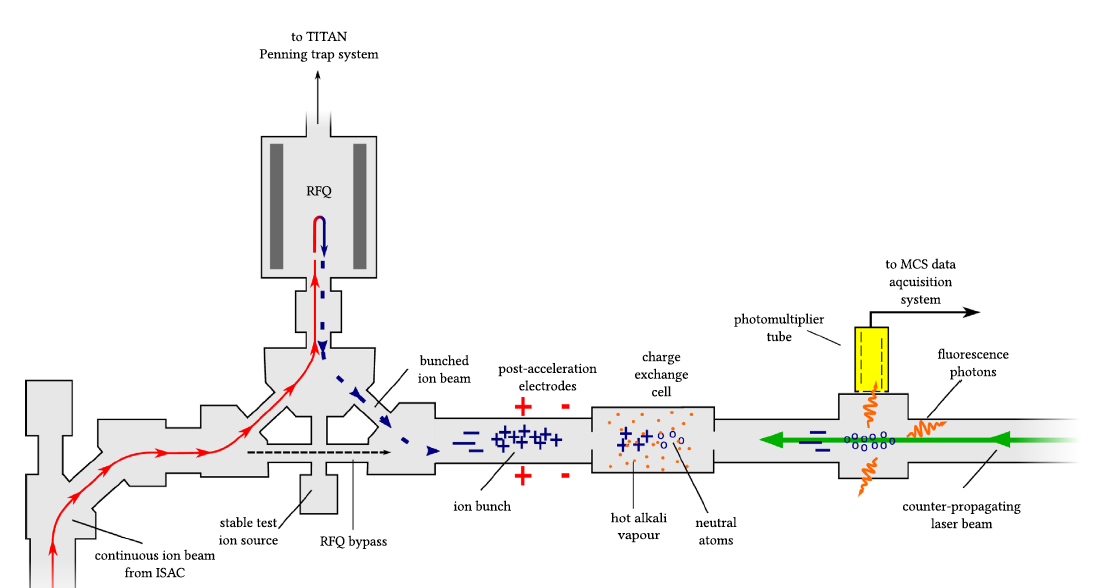
\includegraphics[width=\textwidth]{experiment.png}
\label{exp}
\end{figure}

\section{Optical Pumping}

The distance between the CEC and the LCR introduces the possibility of optical pumping, and effect that can change the ground state distribution of the atoms as they travel the distance between the two regions. This change in ground state distribution is induced by the interaction of the atoms with the laser before they reach the LCR. In an atomic system that has not interacted with a laser, the ground state distribution of the hyperfine levels is statistical (REFERENCE). The likelihood of an electron occupying a hyperfine level with quantum number \textbf{F} is proportional to $F(F+1)$. In a system with N hyperfine levels, each with \textbf{F} = \textbf{F}$_n$, where $n$ = 1,2,3,..N, the probability of an electron occupying, say, the $i$-th level is given by
\begin{equation}
\mathrm{Prob(F}_i) = \frac{F_i(F_i+1)}{\sum_{j=1}^\mathrm{N}F_j(F_j+1)}
\end{equation}

\end{document}